%!TEX root = ../../thesis.tex

\section{Word properties}
\label{chapter:limitations:wordlproperties}


\question{How the world properties (symmetries, size, \ldots) affect the learning properties?}

As discussed in chapter~\ref{chapter:lfui:symmetries}, the properties of the world can affect the learning performances. For example some worlds have symmetric properties which makes some tasks impossible to differentiate. 

In this section, we compare how various planning method perform on our two different worlds, namely the pick and place scenario and the grid world. We will investigate a random strategy, several $\epsilon$-greedy (where the agent follows the best strategy or select an action randomly $\epsilon$ of the times), a strategy based on the task uncertainty (where we do not take the signal to meaning mapping uncertainty in to account), and our uncertainty based method described in chapter\ref{chapter:planning}. We will see that the size of the 

\subsection{Hypothesis and world properties}

Our hypothesis is that the size and optimal policies properties will affect some of the planning method considered more than others. We 

For the pick and place scenario, to reach the correct cube configuration the robot must achieve a very specfic sequence of action in the correct order But for the grid world, a multitude of path can be choosen. 

We will also compares those result with our previous results using a 5 by 5 grid world of chaper~\ref{chapter:planning}

Also for the pick and place scenario, if the signal to meaning mapping were known, to differentiate between two cube configuration that are close together, the agent must go toward those configuration to be able to discard one or an other task. For example, in our illustration of Figure~\ref{fig:lfui:pickplacesequence}, to differentiate between the two first state, one as to reach one of those two states to tell the difference. Indeed, their corresponding optimal policies are similar for every state except their two final states. However for the grid world scenario, if the signal to meaning mapping were known, one could differentiate between the top right state and the state directly on the left of that top right state by simply performing a left action on the bottom right state. And this whatever the size of the grid.

\todo{compute amount of state where optimal polcies differs for two close task}

refer to experiment with pick and place in section lfui and random planning (even if dataset the same after 100 step no confidence) but state space is 625 and no ore 25...

\todo{figure to compare 5x5 and 25x25}

50 run each method each world
90-100 percent datasets

\begin{figure}[!ht]
\centering
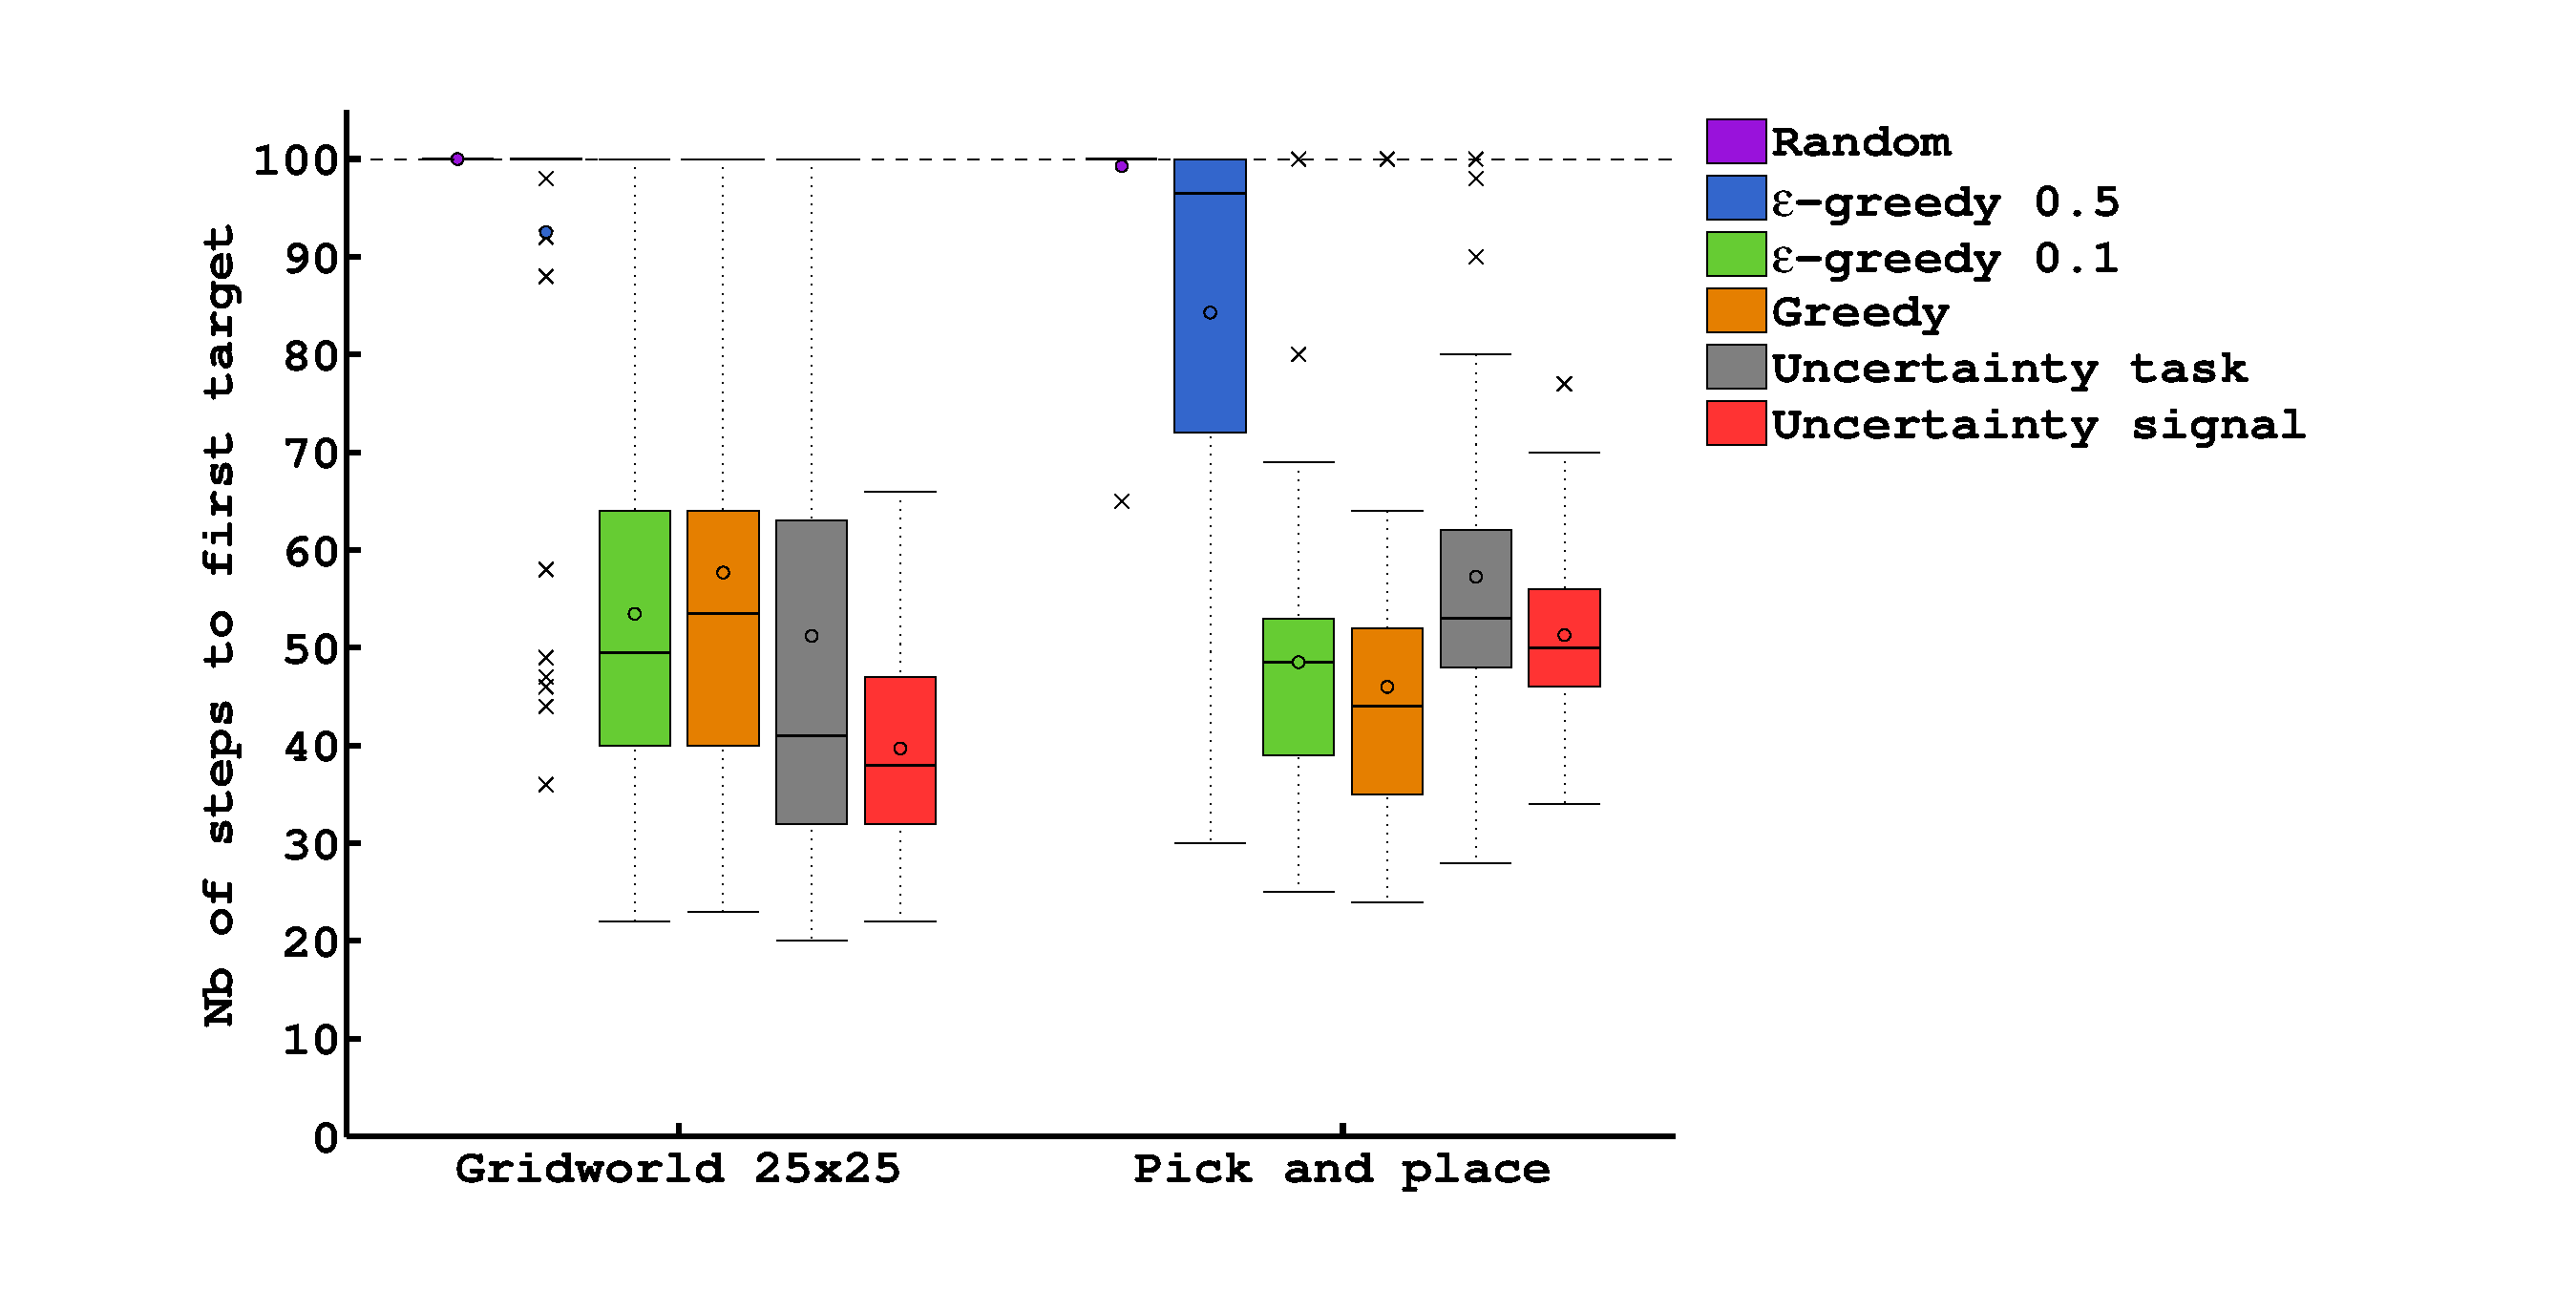
\includegraphics[width=\legendsidesize\columnwidth]{\imgpath/world_properties/firstreach.eps}
\caption{Number of steps to reach first target state with confidence.}
\label{fig:wordlpropertiestimefirst}
\end{figure}

We report only 9 erroneous first task estimations accross all runs of our experiments and conditions.For the gridworld, 1 error for the Greedy method in. For the pick and place scenario, 1 for $\epsilon$-greedy 0.5, 2 for $\epsilon$-greedy 0.1, 2 for Greedy, 1 for Uncertainty task and 2 for Uncertainty signal.

\begin{figure}[!ht]
\centering
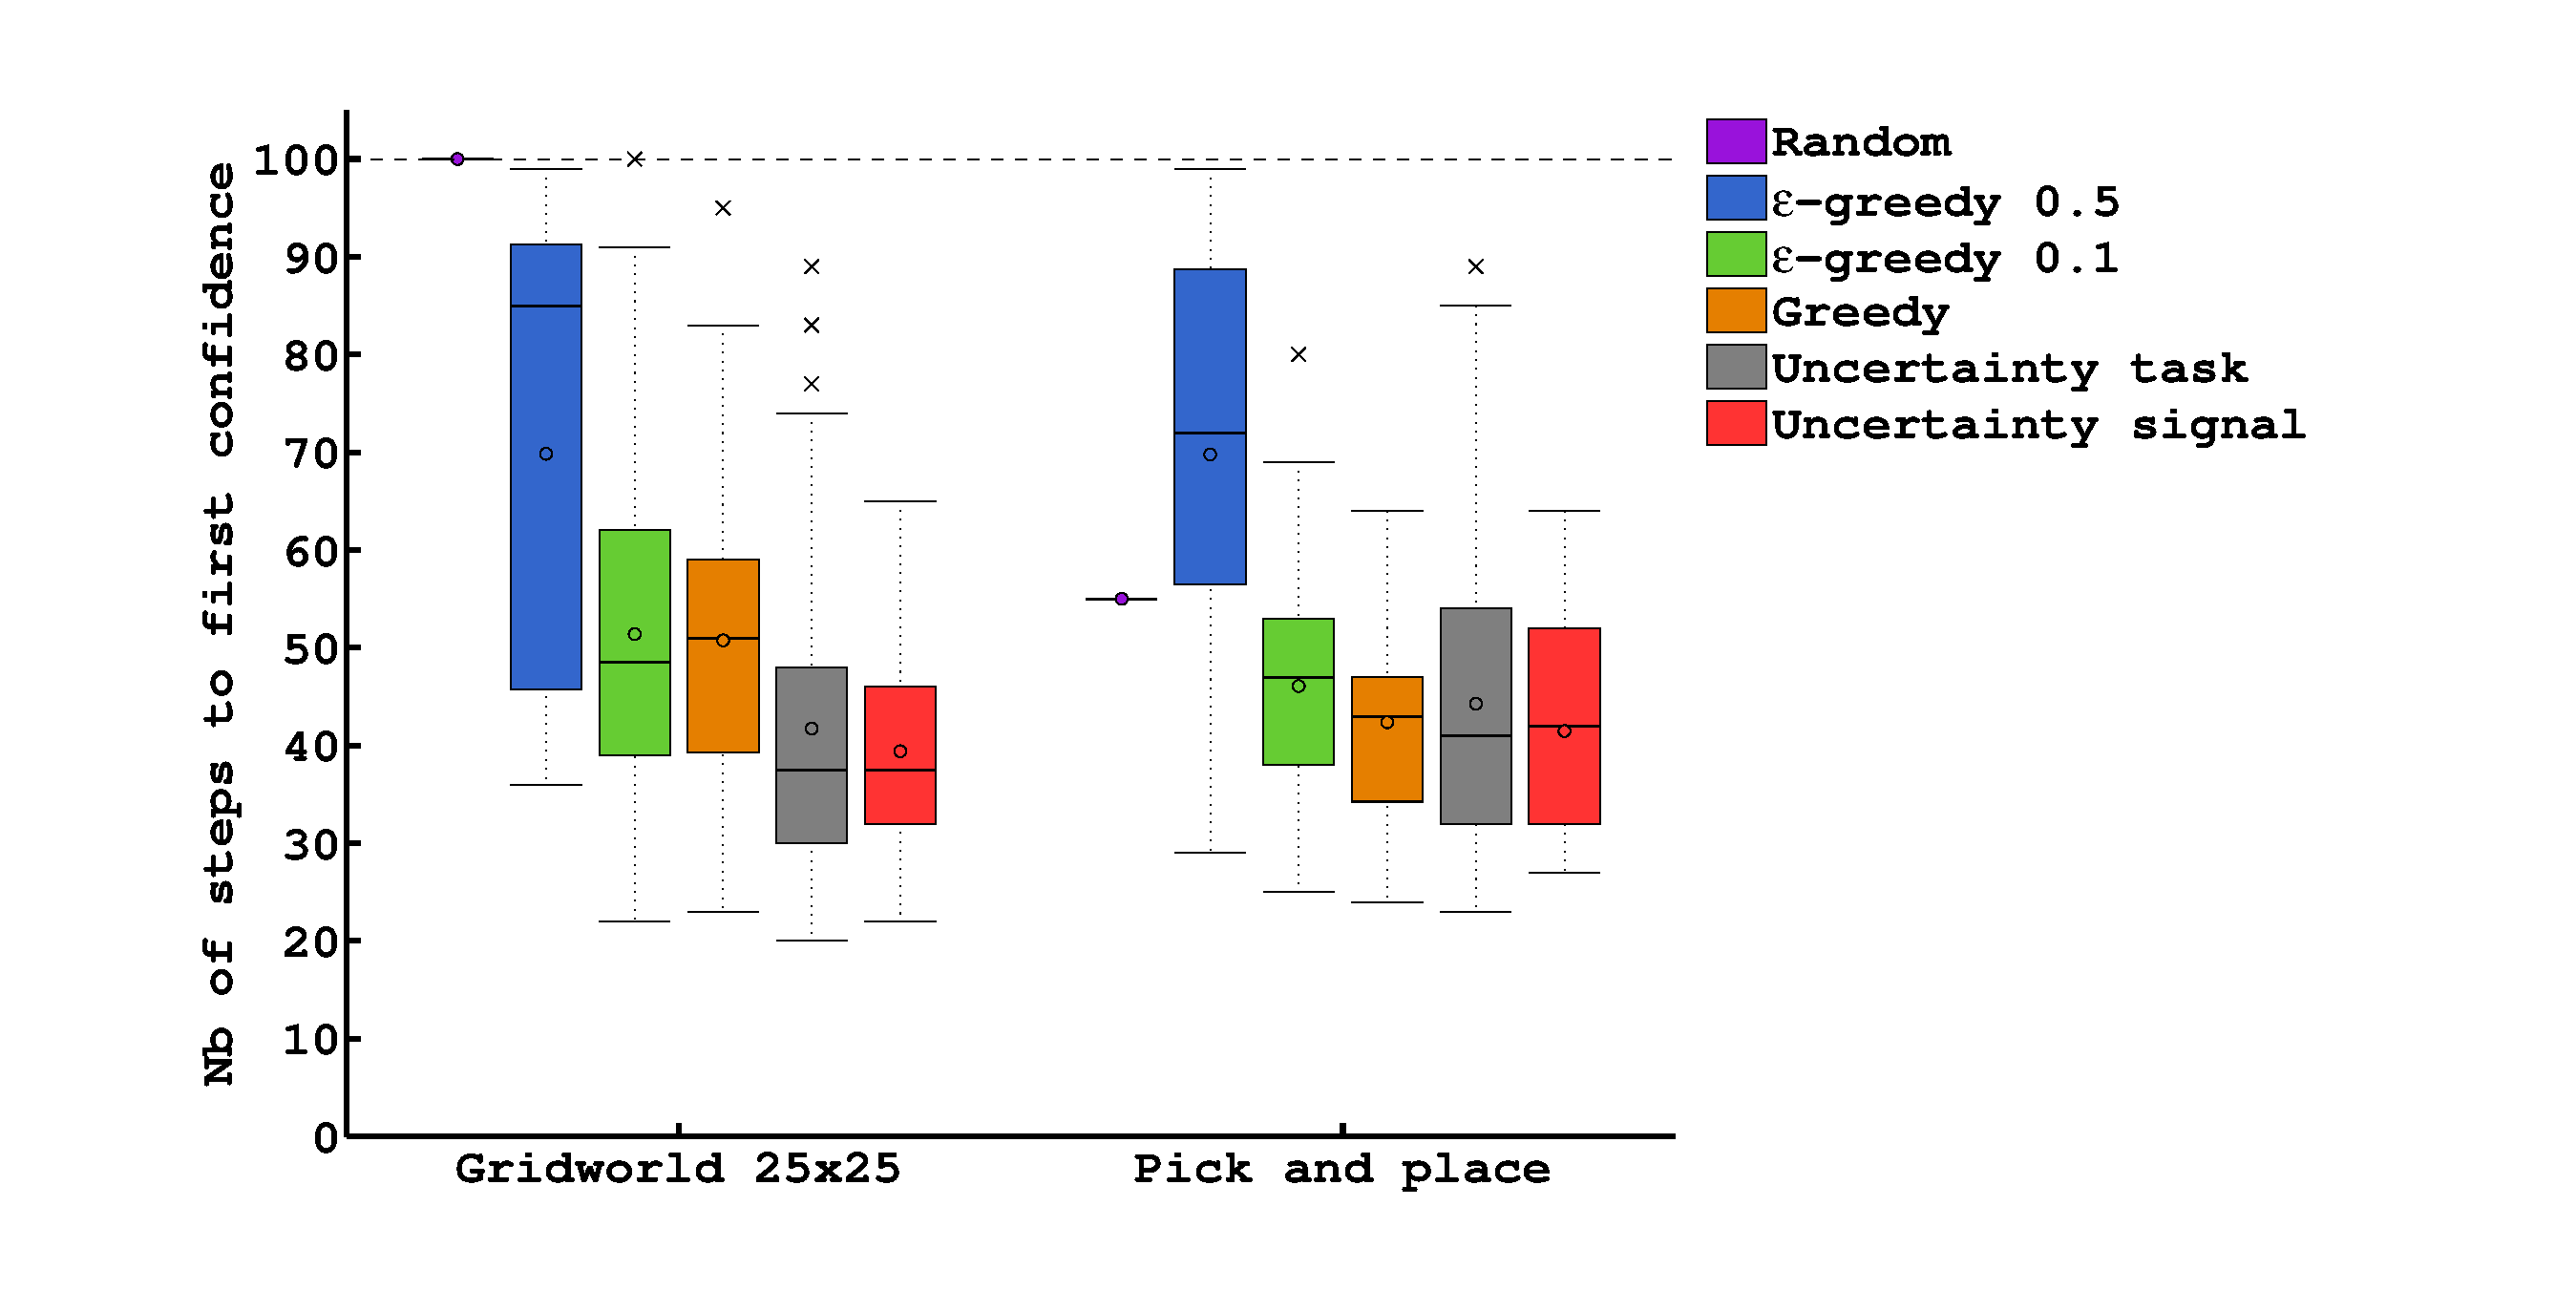
\includegraphics[width=\legendsidesize\columnwidth]{\imgpath/world_properties/firstconfident.eps}
\caption{Number of steps to reach confidence level for the first target.}
\label{fig:wordlpropertiesconfidencefirst}
\end{figure} 

\begin{figure}[!ht]
\centering
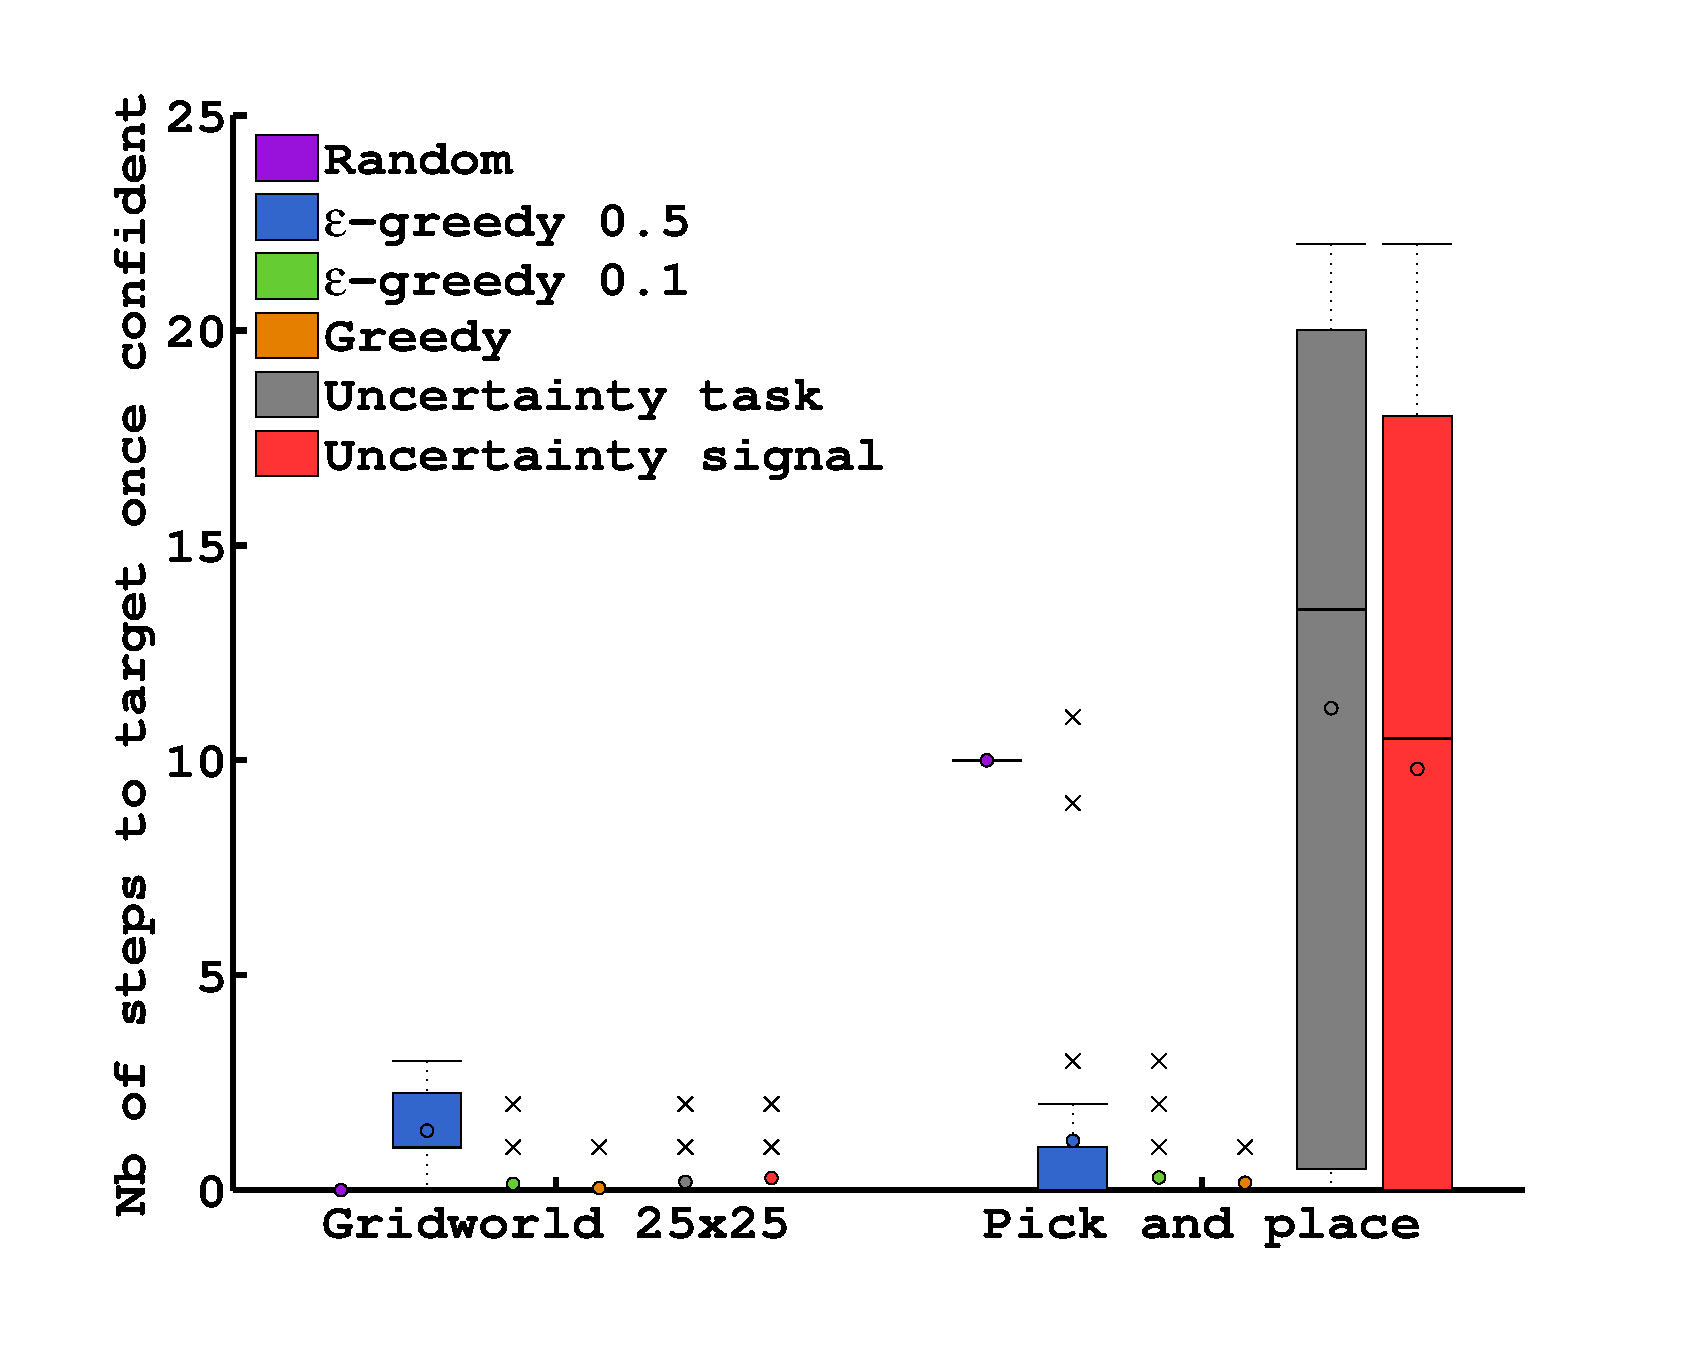
\includegraphics[width=\plotsize\columnwidth]{\imgpath/world_properties/difftargetconfidence.eps}
\caption{Number of action needed to reach the first target when the agent reach confidence level for this target.}
\label{fig:wordlpropertiestargetdist}
\end{figure} 


\begin{table}[!ht]
\centering
\rowcolors{2}{gray!25}{white}
\begin{tabular}{c c c c}
    Planning method & Gridworld &  Pick and place \\ \hline
    Random & 0 & 1 \\ 
    $\epsilon$-greedy 0.5 & 13 & 27 \\
    $\epsilon$-greedy 0.1 & 48 & 48 \\
    Greedy & 43 & 47 \\
    Uncertainty task & 42 & 48 \\
    Uncertainty signal & 50 & 50 \\
\end{tabular}
\caption{Number of experiments that reached at least one target in 100 steps.}
\label{tab:}
\end{table}


conclude by stating difference between end goal learning (graps object, reach state) and reward based learning. We only consider goal learning. episodic (find the right box) vs endless (collect more reward), different exploration function could be used for those

